\documentclass{article}[12pt]
\renewcommand{\baselinestretch}{1.5}

\usepackage[parfill]{parskip}
\usepackage[affil-it]{authblk}
\usepackage[space]{grffile}

\usepackage[a4paper]{geometry}
\geometry{verbose}
\usepackage{float}
\usepackage{graphicx}
\usepackage{setspace}
\usepackage{caption}

\usepackage[utf8]{inputenc}
\usepackage[english]{babel}

\usepackage{latexsym,textcomp,longtable,tabulary}
\usepackage{booktabs,array,multirow}
\usepackage{amsfonts,amsmath,amssymb,mathbbol,calc}
\usepackage{subfigure,color,blindtext,enumitem,siunitx}

\usepackage{mathtools}
\usepackage{url,hyperref,etoolbox}
\numberwithin{equation}{section}
\hypersetup{colorlinks=false,pdfborder={0 0 0}}

%+figure layout options
\restylefloat{figure}
\setlist{leftmargin=*,before=\setlength{\rightmargin}{\leftmargin}}
%-figure layout options

\providecommand\citet{\cite}
\providecommand\citep{\cite}
\providecommand\citealt{\cite}

\setlength{\parskip}{1em}
\makeatletter
\makeatother


\newif\iflatexml\latexmlfalse
\providecommand{\tightlist}{\setlength{\itemsep}{0pt}\setlength{\parskip}{0pt}}%
\AtBeginDocument{\DeclareGraphicsExtensions{.pdf,.PDF,.eps,.EPS,.png,.PNG,.tif,.TIF,.jpg,.JPG,.jpeg,.JPEG}}
\begin{document}

\title{
Field Theory Methods \\
in Reaction-Diffusion Systems
}

\author{Gregory Szep}
\affil{King's College London}
\date{\today}
\maketitle
\vspace{-25pt}
\section{Biochemical Processes as Dynamical Systems} \vspace{-10pt}
In this section we will set the scene for chemical reaction systems and their
methods of analysis from dynamical and topological perspectives. Dynamical
methods makes use of phase space, linear stability and bifurcation analysis.
Green's Functions allow for calculation of correlations and observables.
Graph theory lends insight into the design principles of chemical networks.
Finally a more recent approach to spatiall modelling - moving local equilibria -
is introduced. \vspace{-30pt}
\subsection{Reaction Kinetics} \vspace{-10pt}
Consider $N$ particles of $S$ species in a finite volume $\Omega$. These particles
can undergo $R$ possible reactions when they meet within the volume. Suppose the
timescales of equilibration with respect to volume and temperature are much faster
than that of species number equilibration. This means that non-reactive collisions
occur more frequently than collisions that trigger any of the $R$ reactions.

This suggests that at any time $t$ we may pin down the state of the system by a
vector of populations $s(t)\in\mathbb{N}^S$. The reactions are characterised by
a stoichiometric matrix $\mathbf{\Gamma}\in\mathbb{Z}^{S\times R}$ whos columns
$\gamma\in\mathbb{Z}^{S}$ represent the state change vector for a reaction. Each
reaction also has a propensity $\omega(s|\gamma)\in[0,\infty)$ defined though
probabilities $\mathbb{P}(s,t)$ of being in state $s$ at time $t$.
\begin{align}
	\omega(s|\gamma)\mathrm{d}t := \mathbb{P}(s+\gamma,t+\mathrm{d}t|s,t)
	\label{eq:fundamentalpremise}
\end{align}
Suppose $\sigma(\gamma)\mathrm{d}t$ gives the probability that the state change
$\gamma$ will occur within the time interval $\mathrm{d}t$. The function $\sigma(\gamma)$
could be in principle calculated from the microscopic physics of the reaction.
In quantum mechamics this would involve calculating the wavefunction overlap
or transition rates between initial and final configurations.

This rate is proportional to the propensity, up to combinatoric multiplicity
taking into account the species population $s$. This is the product of all
component pairs $\langle s,\gamma\rangle$ of choosing $|\gamma|$ out of $s$
particles to participate in the reaction.
\begin{align}
	\omega(s|\gamma)=
	\sigma(\gamma)
		\prod_{\langle s,\gamma\rangle}{s \choose |\gamma|}
	\label{eq:propensity}
\end{align}
\subsubsection{Chemical Master Equation}\vspace{-10pt}
By applying the laws of probability and taking the $\mathrm{d}t\rightarrow 0$
one can derive a time-evolution equation $\mathbb{P}(s,t)$ involving
the definition \eqref{eq:fundamentalpremise} which has become known as the
Chemical Master Equation \cite{Gillespie1992,Gillespie2007}.
\begin{align}
	\partial_t\mathbb{P}(s,t) &=
	\sum_{\gamma\in\mathbf{\Gamma}}
	\omega(s-\gamma|\gamma)\mathbb{P}(s-\gamma,t)-\omega(s|\gamma)\mathbb{P}(s,t)
	\label{eq:cme}
\end{align}
Multiplying the Chemical Master Equation \eqref{eq:cme} by $s$ and summing over all $s$
obtains a system of differential equations for the first moment
$\left\langle s \right\rangle$ in terms of vectorised propensity
$\omega(s|\mathbf{\Gamma})\in[0,\infty)^R$ which couples to higher order moments,
unfolding an infinte heirarchy.
\begin{align}
	\partial_t
	\left\langle s \right\rangle &=
	\mathbf{\Gamma} \big\langle \omega(s|\mathbf{\Gamma}) \big\rangle
	\label{eq:momentheirarchy}
\end{align}\vspace{-50pt}
\subsubsection{Reaction Equation}\vspace{-10pt}
The mean field approximation factorises higher order moments, implying
$\big\langle f(s) \big\rangle=f(\langle s\rangle)$ for any nonlinear
function $f$. These fluctuations can be neglected in the $N,\Omega\rightarrow\infty$
thermodynamic limit \cite{Gillespie2007}. This closes the infinite heirarchy
\eqref{eq:momentheirarchy} yielding a nonlinear set of coupled ordinary
differential equations for a continuous vector field $\psi(t)\in[0,\infty)^S$.
\begin{align}
	\partial_t
	\psi &=
	\mathbf{\Gamma}\omega(\psi|\mathbf{\Gamma})
	\label{eq:reaction}
\end{align}
\pagebreak
\subsubsection{Lotka--Volterra Example}\vspace{-10pt}
The Lotka--Volterra model is a canonical example of a predator-prey dynamical
system. Here we may summarise the reactive behaviour between predators $A(t)$
and prey $B(t)$ in Feynman diagrams. Particles are represented by arrows
$\rightarrow$ and reactions by wavy arrows $\leadsto$.
\begin{figure}[H]
\centering{}
\captionsetup{justification=centering}
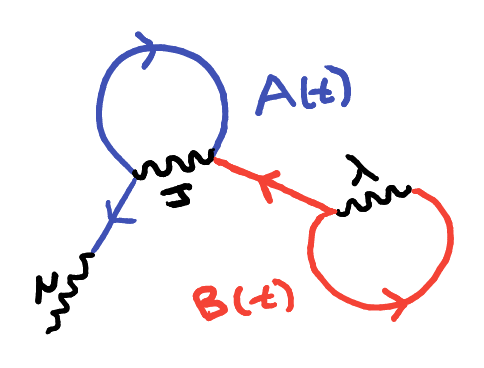
\includegraphics[scale=0.4]{figures/lotkavolterrafield}
\caption{Feynman diagram of the Lotka--Volterra field ${A\choose B\,}$  revealing
autocatalytic birth \\ rate $\lambda$ for prey, constant death rate $\mu$ for predators
and characteristic interaction $J$}
\label{fig:semicircle}
\end{figure}
Letting $s(t)={A\choose B\,}$, the stoichiometric matrix $\mathbf{\Gamma}$ and
propensity $\omega(s|\mathbf{\Gamma})$ are determined from the state changes
$\gamma$ and the rates of each reaction.
\begin{align}
	\mathbf{\Gamma}=
	\begin{pmatrix}
		-1 & 0 & 1 \\
		0 & 1 & -1 \\
	\end{pmatrix}
	\qquad\qquad
	\omega(s|\mathbf{\Gamma})=
	\begin{pmatrix}
	  \mu A(t)\\
		\lambda B(t)  \\
		J A(t)B(t) \\
	\end{pmatrix}
\end{align}
\subsection{Reaction Topology}

\subsection{Reaction-Diffusion}

\section{Field Theory Approach}
\subsection{Master Equation}

\subsection{Path Integrals}

\subsection{Green's Functions}
\bibliography{bibliography/biblio}
\bibliographystyle{ieeetr}
\end{document}
